
\begin{figure*}[t!]
    \centering
    \begin{subfigure}[b]{0.36\textwidth}
        \centering
        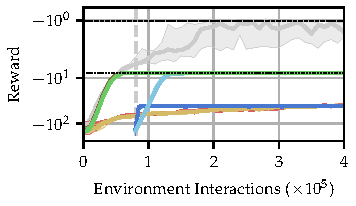
\includegraphics[width=\textwidth]{figures/sec4/cr/lg/sec4_results_IceLake_True_cr_logs_LavaGap_LavaGapCompiledRun_.pdf}
        \caption{Frozen Lake.}
        \label{fig:gridworld_asym:IceLake}
    \end{subfigure}%
    \hfill
    \begin{subfigure}[b]{0.36\textwidth}
        \centering
        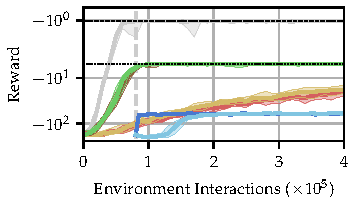
\includegraphics[width=\textwidth]{figures/sec4/cr/td/sec4_results_TigerDoor_True_cr_logs_TigerDoor_TigerDoorCompiledRun_.pdf}
        \caption{Tiger Door.}
        \label{fig:gridworld_asym:TigerDoor}
    \end{subfigure}%
    \hfill
    \begin{subfigure}[b]{0.18\textwidth}
        \centering
       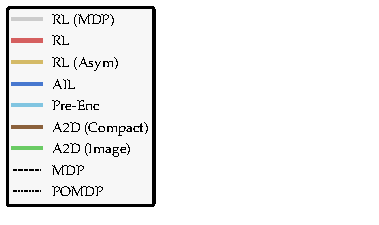
\includegraphics[width=\textwidth]{figures/sec4/legend_sec4_results.pdf}
    \end{subfigure}
    \caption{Results for the gridworld environments.  Median and quartiles across $20$ random seeds are shown.  TRPO~\citep{schulman2015trust} is used for RL methods.  Broken lines indicate the optimal reward, normalized so the optimal MDP reward is $-1$ (\emph{MDP}).  All agents and trainees are conditioned on a image-based input, except \emph{A2D (Compact)} which is conditioned on a partial compact state representation.  All experts, and \emph{RL (MDP)}, are conditioned on an omniscient compact state.  \emph{Pre-Enc} uses a fixed pretrained image encoder, trained on examples from the MDP.  \emph{AIL} and \emph{Pre-Enc} begin when the MDP has converged, as this is the required expenditure for training.  A2D is the only method that reliably and efficiently finds the optimal POMDP policy, and, in a sample budget comparable with \emph{RL (MDP)}.  The convergence of A2D is also similar for \emph{both} image-based (\emph{A2D (Image)}) and compact (\emph{A2D (Compact)}) representations, highlighting that we have effectively subsumed the image perception task.  Configurations, additional results and discussions are included in the appendix.}
    \label{fig:gridworld_asym}
\end{figure*}
